\documentclass[pdflatex,sn-nature,oneside]{sn-jnl}

\usepackage{graphicx}
\usepackage{amsmath,amssymb}
\usepackage{booktabs}
\usepackage{xcolor}
\usepackage{hyperref}

\raggedbottom

\begin{document}

% ─────────────────────────────────────────────────────────────────────────────
% TITLE & AUTHORS
% ─────────────────────────────────────────────────────────────────────────────

\title[What would make biodiversity offset markets work across all ecosystem types?]%
      {What would make biodiversity offset markets work across all ecosystem types?}

\author*[1]{\fnm{José Luis} \sur{Reséndiz}}\email{jose.resendiz@smithschool.ox.ac.uk}

\affil*[1]{\orgdiv{Smith School of Enterprise and the Environment},
           \orgname{University of Oxford},
           \orgaddress{\city{Oxford}, \postcode{OX1 3QY}, \country{UK}}}

% ─────────────────────────────────────────────────────────────────────────────
% ABSTRACT
% ─────────────────────────────────────────────────────────────────────────────

\abstract{%
Biodiversity offset markets are meant to compensate, ecosystem by
ecosystem, for habitats that development destroys. Do they? We
analyse 1,124 transactions from Australia's largest mandatory offset
scheme. Across 252 ecosystem types in the scheme, only 18\% sustain
a working market, and 47\% of the threatened communities the scheme
is designed to protect receive no direct investment at all. The reason
is structural: buyers minimise cost, demand concentrates on a handful
of cheap types, and developers route obligations through a government
fund rather than purchasing credits directly. An agent-based model
that reproduces this gap shows what would help. Restricting fund pay-in
and requiring buyers to direct some demand toward underserved types
raise coverage at modest cost; minimum prices and tighter government
procurement rules do not. Markets that share this design risk the same
failure unless procurement rules are rewritten.%
}

\keywords{biodiversity offsets, ecological coverage,
          vegetation formations, competitive exclusion,
          procurement flexibility, biodiversity net gain}

\maketitle

% ─────────────────────────────────────────────────────────────────────────────
% INTRODUCTION
% ─────────────────────────────────────────────────────────────────────────────

Biodiversity offset markets exist so that when development damages an ecosystem,
the developer compensates by funding protection or restoration elsewhere.
As of 2023, mandatory offset schemes transact an estimated \$11.7 billion per
year~\cite{UNEP2023}, with nineteen national and subnational schemes operational
or in development across six continents~\cite{IAPB2024}.
Within each, a developer who damages a protected habitat or species must buy
credits from a landholder who protects or restores an equivalent ecosystem
elsewhere.
Credits are specific to ecosystem type: a developer who clears woodland
must buy woodland credits. The number and boundaries of these types are
fixed by the regulator through official ecosystem classification lists,
fragmenting each scheme into hundreds of separate sub-markets.
Because vegetation communities differ vastly in their spatial extent, landholder
willingness, and restoration feasibility, the supply of credits varies
dramatically across ecosystem types.
The question is not whether these markets should be linked to development
(that is their purpose) but whether they deliver
compensation evenly across the ecosystem types they are mandated to protect.
A 2019 global review of biodiversity offset schemes found that only
approximately one-third achieved no-net-loss outcomes~\cite{zuErmgassen2019}.
These failures have been attributed primarily to metric design, monitoring gaps,
and political compromise~\cite{Gibbons2018,Maron2016}, but whether the market design itself systematically excludes
most ecosystem types from receiving investment remains an open question.

There are theoretical reasons to suspect it does.
Compliance buyers must offset impacts on a specific ecosystem type, but when
their obligation can be met by credits from related types within the same
vegetation formation, they minimise cost.
Drechsler~\cite{Drechsler2024} predicted that this will concentrate demand in
commercially accessible types, and zu Ermgassen et al.~\cite{zuErmgassen2020}
argued that the resulting loss of scarcity signals undermines impact avoidance.
But neither prediction has been tested with transaction-level data, and the
role of developers routing demand through a government fund, rather than
purchasing directly, has not been examined.

We test this using transaction-level data from the New South Wales (NSW)
Biodiversity Offsets Scheme, Australia's largest mandatory offset market
(AUD\,105M annual turnover~\cite{IPART2024}), operational since 2017
and recording over 1,100 credit transactions across 252 ecosystem types.
The scheme recognises 252 distinct ecosystem credit types, each corresponding
to a specific vegetation community.
Transaction data alone reveals that 112 of these 252 types (44\%) have never
been traded, but cannot explain why or predict which interventions would help.
For that, we build an agent-based model in which four participant species
interact across these credit types. Following Farmer's market-ecology
framework~\cite{Farmer2002,SchollCalinescuFarmer2021}, species are defined
by behavioural strategy rather than by institutional identity:
(i) cost-minimising compliance demand: agents seeking the cheapest credit
that satisfies their obligation;
(ii) mean-reversion intermediation: agents bidding against rolling
fundamental value to exploit price dispersion;
(iii) thin-market procurement: budget-constrained agents that bid above
the compliance median in low-liquidity types to ensure coverage;
(iv) cost-floor supply: credit producers who sell only when market price
exceeds a fraction of marginal production cost.
In NSW these strategies are realised by, respectively, compliance buyers
(i), intermediaries (ii), the Biodiversity Conservation Trust (BCT) (iii)
drawing on the Biodiversity Conservation Fund (the Fund), and habitat
banks (iv) (landholders who generate and sell credits).
The model identifies three reinforcing mechanisms that explain why most
ecosystem types are left without a functioning market, defined here
as one with enough repeated transactions for buyers to reliably find
a willing seller.
First, compliance buyers select the cheapest available credit type, concentrating
demand in a few well-supplied types (least-cost selection).
Second, when buyers cannot find credits for their specific obligation, they pay
into the Fund rather than purchasing directly, routing demand
away from the types that need it most (fund routing).
Third, credit types that have traded before are approximately 8.4 times more
likely to trade again, creating a self-reinforcing cycle in which popular types
attract more demand while neglected types remain neglected (liquidity feedback).

Our model, which incorporates these three mechanisms alongside
realistic agent behaviour and market structure, reproduces the
observed pattern: most ecosystem types lack a functioning market.
Because the model captures the mechanisms that generate the gap, we can
use it to test which policy changes would close it.
We evaluate five interventions, each targeting a different mechanism,
and measure their effect and cost on \emph{functional coverage}, the
fraction of ecosystem types sustaining a functional market
($\geq$5 transactions).
The most effective interventions are those that keep demand in the open
market: restricting developers' access to the Fund (bypass
reduction) and requiring a fraction of purchases to be directed toward
underserved types (procurement flexibility).
Unlike the buyer-choice flexibility that previous work has shown to erode
scarcity signals~\cite{zuErmgassen2020}, these are regulator-directed
instruments that preserve price signals while channelling new demand where
it is absent.
Interventions that restrict flexibility or raise costs without redirecting
demand, including setting minimum credit prices (price floors),
requiring more credits for rare types (rarity multipliers), and
mandating exact like-for-like matching for BCT purchases
(BCT precision mandate), are ineffective or counterproductive.
Because these policy conclusions could depend on how the model is built,
we validate the results out of sample using a temporal split (calibrating
on pre-2024 data and predicting post-2024 outcomes) and confirm them with
an independent analytical model based on ecological competition theory.

The design failure documented here is not confined to NSW\@.
At least nineteen national and subnational biodiversity offset schemes are
operational or in development worldwide, including the United Kingdom's
Biodiversity Net Gain framework, which became mandatory in 2024~\cite{IAPB2024}.
Each operates a compliance market in which developers offset impacts on
specific ecosystem types, and each faces the same structural risk: that
least-cost compliance will concentrate demand before coverage gaps can be corrected.
The NSW evidence shows that once the liquidity feedback cycle has set in,
the pattern is self-reinforcing.
The intervention window is open now, before these markets lock in the same design.


% ─────────────────────────────────────────────────────────────────────────────
% RESULTS
% ─────────────────────────────────────────────────────────────────────────────

\section{Results}\label{sec:results}

\subsection*{Most ecosystem types lack a functioning market}

Analysis of 1,124 priced transactions from the NSW Biodiversity Offsets Scheme
public register (November 2019--March 2026) reveals a coverage gap.
The Scheme recognises 252 distinct ecosystem credit types (offset trading groups,
OTGs).
Of these, 140 (56\%) have recorded at least one priced transaction;
the remaining 112 (44\%) have never been traded.
Only 45 (18\%) have traded often enough to sustain what we term a
\emph{functional market}: five or more transactions over the observation
period, a conservative threshold below which transaction frequency is too low
for reliable price discovery~\cite{Cont2001} (Fig.~\ref{fig:problem}a).
We define \emph{functional coverage} as the fraction of ecosystem types that
clear this threshold.
This gap is persistent, not transient: among ecosystem types below the
functional threshold, transaction counts remain near zero across six
years of data, and no individual credit type shows a meaningful trend
toward viability.
The market is not self-correcting.

This coverage gap is not explained by the absence of potential supply:
all 252 ecosystem types have registered landholders, confirming that
credits could be generated if demand existed at viable prices.
Nor is it explained by absent demand. Developers do incur offset
obligations in rare credit categories, but instead of purchasing credits
directly, they pay into the Fund, and the Trust purchases on their
behalf. The 24 credit categories served only by the Trust have each
received at least one such indirect purchase, consistent with developer
demand existing for these types but being routed away from the open
market via the Fund.

The exclusion is systematic, not random.
Of the 252 ecosystem credit types, 79 correspond to listed Threatened
Ecological Communities (TECs) and 173 to non-TEC vegetation types.
Because offset obligations reference TECs by name, compliance demand
flows disproportionately toward listed communities: TECs are
significantly more likely than non-TECs to record at least one transaction,
and under strict name-matching no non-TEC type appears in the priced-transfer
register at all (Methods).
But even this directed demand is insufficient.
Of the 79 listed threatened communities, 47\% receive no direct market
investment: 31 have never been traded and 6 have been purchased only by
the conservation Trust using Fund money, not by any compliance buyer on
the open market.
Only 18 sustain functional markets: the scheme fails to deliver
reliable compensation for more than three out of every four threatened
communities it lists.

The scale of fund routing is substantial.
Of 1,097 credit retirements, 35\% were Trust purchases on behalf of
developers who paid into the Fund rather than purchasing credits
directly~\cite{IPART2024}.
Buyer concentration reinforces the pattern.
The Herfindahl-Hirschman Index (HHI) reached 2,966 in 2024--25 (above the 2,500
threshold for highly concentrated markets), up from 2,187 the prior
year~\cite{IPART2025} (Fig.~\ref{fig:problem}b).
The scheme does have a backstop for ecosystem types that the open market
fails to serve, but as the next section shows, that backstop is itself
under pressure.

\subsection*{The government backstop does not close the gap}

The Biodiversity Conservation Trust (BCT, hereafter the Trust) is the
NSW government agency responsible for investing in private land
conservation. When developers cannot find credits in the open market
for their specific ecosystem type, they can pay into the Fund and
transfer the obligation to the Trust, which procures credits on their
behalf. This makes the Trust the de facto safety net for thin-market
ecosystem types: for 24 credit categories, it is the only buyer that
has ever purchased credits.
The discretion produces a measurable price premium: in thin markets
(fewer than five lifetime transactions), the Trust pays a median of
AUD\,5,989 per credit versus AUD\,1,125 for direct compliance buyers,
a 5.3-fold differential that is highly significant (Methods).
In functional markets the differential is markedly
smaller, confirming that the premium reflects the Trust's role in
thin markets rather than an artefact of overall price levels.

But this safety net is weakening. The Trust's share of credits more
than doubled from 7\% in 2022--23~\cite{IPART2023} to 16\% in
2024--25~\cite{IPART2025}, yet the fraction of its purchases matching
the specific credit type required by the underlying developer obligation
(the like-for-like rate) fell from 90\% to 65\% over the same period. If
volume growth comes at the cost of reduced like-for-like precision, the
Trust may be processing Fund-routed demand rather than directing
procurement toward conservation targets, and the 24 rare credit
categories that depend on exact matching go unserved. A developer who
damages Coastal Upland Swamp pays into the Fund expecting compensation
for that specific community; the Trust may instead procure credits from
a more readily available type, leaving the original ecosystem
uncompensated.

The transaction data reveal what is happening but not why, nor which
interventions could improve outcomes. We test five: restricting developers'
access to the government fund, redirecting a fraction of demand toward
underserved types, requiring higher credit quantities for rare ecosystem
types, setting a minimum credit price, and mandating exact matching for the
government procurement agency.
Together these target each component of the coverage gap from both the
demand and supply sides.

\subsection*{Keeping demand in the open market is the most effective intervention}

To test whether the observed coverage gap arises from market structure
rather than idiosyncratic factors, we built an agent-based model of the
NSW scheme: 252 ecosystem credit types grouped by 15 vegetation formations
across 40 ecological subregions, with four kinds of participant:
compliance buyers (cost-minimising), intermediaries (profit-seeking), the
Trust (procurement-flexible), and habitat banks (credit suppliers). The
model incorporates a self-reinforcing demand-concentration mechanism in
which credit types that have traded before attract more demand, with
weights estimated directly from the NSW transaction register: types
with $\geq$10 prior transactions are 8.4$\times$ more likely to be chosen
than untraded types (Methods). All other parameters are derived from
data; one parameter (the rate at which compliance buyers attempt
within-formation substitution) is calibrated to match the observed Fund
routing rate.

The model reproduces the empirical coverage gap. Functional coverage in
the model is 16.3\% (median across 50 Monte-Carlo runs; observed: 17.9\%),
the simulated and observed shares of transactions across vegetation
formations are tightly correlated (Methods, Fig.~\ref{fig:mechanism}a),
and the simulated split of retirements between compliance buyers and the
Trust (65.8\%/34.2\%) reproduces the observed 65\%/35\% breakdown. Five
formations that are empirically near-extinct in the data (Grasslands,
Rainforests, Saline Wetlands, Arid Shrublands, and Heathlands; each
$\leq$9 lifetime transactions) emerge as near-extinct in the model
without being targeted by calibration.

We test five policy interventions, each targeting a different component
of the coverage gap (Table~\ref{tab:scenarios}; Fig.~\ref{fig:mechanism}b).
Only two of the five interventions improve coverage relative to baseline
(16.3\%), and both work by keeping demand in the open market rather than
diverting it to the Fund. Bypass reduction (making it harder for
developers to pay into the Fund) raises functional coverage to 17.5\%
and cuts Fund routing from 34.1\% to 21.3\%. Procurement flexibility
mandates (requiring compliance buyers to direct 20\% of purchases
toward thin-market types) raise coverage to 17.1\%.
Three interventions fail. Price floors (AUD\,3,000 minimum) push more
developers into the Fund (routing rises to 50.5\%) without generating
new direct demand. Mandating exact like-for-like matching for the
Trust's purchases is actively counterproductive (coverage falls to
12.7\%): the Trust can no longer procure credits when the exact ecosystem
type has insufficient supply, and damage falls disproportionately on
threatened communities (in the model, FC-TEC drops from 25.3\% to 16.5\%,
eliminating a third of the functional TEC markets in simulation;
empirical FC-TEC is 22.8\%). The rarity multiplier (2$\times$ credits required for rare
types) has only a marginal effect (16.5\%), confirming that the
bottleneck for rare types is the existence of demand, not the quantity
per transaction. One formation (Arid Shrublands, Acacia sub-formation)
remains market-extinct under all scenarios: its development pressure is
so low that no demand-side intervention generates obligations there.

\subsection*{Robustness}

The conclusions are robust to specification, sample, and modelling
framework~\cite{Fagiolo2007}. Calibrated to a single observable (the
35.4\% Fund routing rate), the model reproduces three other empirical
patterns it was not calibrated to: the headline coverage gap, the
compliance/Trust split of retirements, and the dominance of Grassy
Woodlands. The formation-level ranking is preserved under both
a within-sample temporal split (pre-2024 vs 2024--26) and a formation
hold-out (excluding Grassy Woodlands from calibration). Parameter
sensitivity confirms that functional coverage moves by less than one
percentage point when any parameter is perturbed across a six-fold
range; the only exception (the number of Trust agents, 5.4\,pp) does
not change the scenario \emph{ranking}. A separate analytical model
based on Generalised Lotka--Volterra ecological dynamics, calibrated to
the same data but solved as differential equations rather than agent
simulation, identifies the same most- and least-effective interventions
(Supplementary Note~1; Supplementary Fig.~1a--b; Supplementary Table~6).


% ─────────────────────────────────────────────────────────────────────────────
% DISCUSSION
% ─────────────────────────────────────────────────────────────────────────────

\section{Discussion}\label{sec:discussion}

\textbf{Intervention hierarchy.}
The five policy scenarios test interventions targeting each component of the
coverage gap. Two clear lessons emerge.
First, the most effective interventions are those that keep demand within
the open market rather than diverting it to the Fund.
Bypass reduction (functional coverage 17.5\%) and procurement flexibility
(17.1\%) both work by increasing the probability that a compliance buyer
transacts directly with a credit supplier, rather than paying into a
government fund.
This finding converges with the NSW regulator's own assessment:
IPART~\cite{IPART2023} independently concluded that the Fund pay-in
option prevents the market from developing and recommended phasing it
out. Our model quantifies why: every obligation that enters the Fund
is one fewer direct transaction in the open market, and the cumulative
effect is a 13 percentage point reduction in Fund routing (from
34.1\% to 21.3\%) when bypass is restricted.

Bypass reduction operates as a necessary precondition rather than a
stand-alone fix. The 2024 Amendment Act acquittal deadline reduced NSW
market bypass from 81\% in 2022--23 to approximately 18\% in
2024--25~\cite{IPART2025}, while functional coverage held at 18\% over
the same window (Supplementary Table~1 footnote): bypass reduction
redirects demand toward the open market, and procurement flexibility ---
which allocates a share of compliance demand to underserved types ---
translates that redirected flow into coverage gains.

The US 2008 Final Rule~\cite{USFinalRule2008} reached a similar
conclusion for wetland mitigation, establishing a preference hierarchy
(mitigation banking $>$ in-lieu fee) after a decade of evidence that
fund-based mechanisms delivered weaker ecological
outcomes~\cite{HoughHarrington2019}.
The closest precedent for procurement flexibility mandates is technology
carve-outs in Renewable Portfolio Standards, where mandating minimum
purchases from specific energy types increased technology diversity
even when general portfolio targets did not~\cite{KimTang2020}.

Second, interventions that restrict flexibility or raise costs without
redirecting demand are ineffective or counterproductive.
Price floors cause developers to route more obligations into the Fund
(routing rate from 34.1\% to 50.5\%) without generating new direct
demand~\cite{WoodJotzo2011}.
Mandating exact like-for-like matching for BCT purchases reduces coverage
to 12.7\%, confirming that government intermediaries need procurement
flexibility to serve thin markets~\cite{VanTeeffelen2014}.
The rarity multiplier (2$\times$ credits for rare OTGs) has negligible
effect (16.5\%) because the bottleneck for underserved types is the
existence of demand, not the quantity per transaction; this is
consistent with the theoretical finding that uniform multipliers
are inadequate for rare habitats~\cite{Bull2017multipliers}.

zu Ermgassen et al.~\cite{zuErmgassen2020} argued that relaxing
like-for-like rules destroys the scarcity signal that incentivises
impact avoidance, and Drechsler~\cite{Drechsler2024} showed formally that
buyer-choice flexibility always reduces ecological benefit.
Our data provide empirical evidence consistent with this prediction.
The procurement flexibility mandate does not relax like-for-like rules for
the buyer; instead, regulators direct a fraction of compliance demand toward
underserved types, preserving the scarcity signal for the remaining 80\% of
purchases while channelling new demand where it is absent.
Bypass reduction and procurement flexibility therefore constitute
the core policy package for improving ecological coverage. Both can be
implemented within existing statutory frameworks.

\textbf{Why these interventions work: three layers of exclusion.}
The effectiveness of demand-side interventions reflects the depth of the
coverage gap, which operates at three levels.
First, non-TEC vegetation types (the ecological matrix that provides
connectivity and buffering for threatened
patches~\cite{Driscoll2013,FischerLindenmayer2007}) receive systematically
less direct market investment than listed TECs, because offset obligations
reference TECs by name (Methods).
Second, even when an obligation does fall on a TEC, current rules let
the offset be discharged outside the open market: offset obligations
capture only direct clearing impacts, while supply-chain, cumulative,
and diffuse impacts remain uncompensated~\cite{Mace2012}.
Third, and most critically, the market fails even within its own intended
scope: 47\% of listed TECs receive no direct market investment (37 of 79
have never traded or are served only by the Trust), and the 24 ecosystem
types served only by the Trust show that developers route demand through
the Fund rather than the open market.
The market is failing on its own
terms~\cite{MacKenzie2006performative}: designed to compensate for
development impacts on listed threatened communities, it instead channels
investment toward the most commercially accessible types. zu Ermgassen
et al.~\cite{zuErmgassen2020} noted that the 2017 Biodiversity
Conservation Act places no legal restriction on the Trust offsetting
using any habitat type anywhere in the state; our data quantify the
consequence. The Trust's budget (AUD\,47.3M per year) is sufficient to
sustain market activity in all but one formation, yet five are empirically
near-extinct, consistent with the Trust's declining like-for-like
precision (90\%$\to$65\%).

\textbf{Costs and implementation.}
Cost-effectiveness --- private outlay per percentage point of functional
coverage gained --- is modest under the effective interventions. Bypass
reduction increases total market expenditure by 3.1\% and procurement
flexibility by 0.6\% (Supplementary Table~8), with average credit prices
essentially unchanged. The Trust's procurement load follows the Fund
routing rate: bypass reduction shifts routing from 34.1\% to 21.3\%,
reducing regulator outlay; price floors increase routing to 50.5\% and so
raise the regulator's burden even where private cost is flat. By
comparison, a 20\% solar carve-out in US Renewable Portfolio Standards
increased programme costs by 28\%~\cite{NovacheckJohnson2015}.
A striking asymmetry emerges: it is far easier to damage coverage than
to improve it. The BCT precision mandate reduces coverage by 3.6
percentage points (eliminating a third of functional TEC markets),
while the best positive intervention (bypass reduction) gains only 1.2
percentage points. This asymmetry implies that poorly designed
procurement rules can cause irreversible coverage losses that even
well-designed interventions struggle to reverse.
Flexibility mandates also raise acquittal complexity for developers, and the
20\% threshold invites gaming near the margin.
An alternative route to the same goal is to embed coverage
directly into the credit metric itself, for example through
irreplaceability-weighted credits that assign higher value to
underrepresented habitat types~\cite{Bush2024}.
Functional coverage should become an explicit regulatory
metric~\cite{Needham2019}, monitored alongside volume and price, to provide an
operational early warning of coverage decline before it becomes irreversible.

\textbf{Generalisability and limitations.}
The demand-concentration mechanism is not unique to biodiversity markets:
analogous coverage biases have been documented in renewable energy
markets~\cite{ZhouSolomonBrown2024,Bjorn2022} and water entitlement
markets~\cite{DonnaEspinSanchez2026,Connor2013}, where mandatory or
compliance-driven demand also concentrates on the cheapest types. The
mechanism here is therefore structurally general, but the quantitative
findings are NSW-specific: every parameter is calibrated to NSW data, and
the four-participant typology presupposes a compliance-buyer population,
an exogenous-mandate demand structure, a government safety-net agency,
and credit-type segmentation. These design features describe most
current compliance offset schemes, including the United Kingdom's
Biodiversity Net Gain framework, but transferring quantitative numbers to
markedly different designs would require recalibration.

The scenario ranking
(Bypass Reduction $>$ Procurement Flexibility $>$ Rarity Multiplier
$\geq$ Baseline $>$ Price Floor $>$ BCT Precision Mandate) holds across
the parameter ranges examined in Supplementary Table~6 and the global
sensitivity analysis in Supplementary Note~2.

Functional coverage in this analysis is an outcome metric tied to the
regulator's stated intent --- every listed ecosystem type should sustain
a market --- rather than a welfare measure integrating ecological benefit
against fiscal cost; the ranking reports how well each intervention
satisfies the scheme's compensatory design. Scenario-comparison
percentiles overlap by approximately one percentage point, so the
ranking is ordinal in the small-difference range. The next test of
generalisation comes from the United Kingdom's Biodiversity Net Gain
framework, which became mandatory in 2024.
Making biodiversity offset markets work across all ecosystem types requires
procurement rules that keep demand in the open market rather than rewarding
cost minimisation.
For NSW and every market that follows it, the intervention window remains open,
the policy tools are identified, and the statutory authority to act already exists.


% ─────────────────────────────────────────────────────────────────────────────
% ONLINE METHODS
% ─────────────────────────────────────────────────────────────────────────────

\section*{Online Methods}\label{sec:methods}

\textbf{Market ecology framework.}
The market ecology framework treats financial market participants as biological
species competing for limited profit opportunities, with population dynamics governed
by the profitability of their behavioural
strategies~\cite{Farmer2002,SchollCalinescuFarmer2021}.
The framework extends the ecological metaphor of Lo's Adaptive Markets
Hypothesis~\cite{Lo2004} into a formal dynamical system, drawing on earlier
applications of ecological network theory to financial stability~\cite{HaldaneMay2011,
MayLevinSugihara2008}.
We build on the formulation of Scholl, Calinescu, and
Farmer~\cite{SchollCalinescuFarmer2021}, who showed that the ecological community
matrix of interacting trading strategies can be computed numerically from a Walrasian
agent-based model.
We use Generalised Lotka-Volterra (GLV) equations as an analytically tractable
complement to the ABM, validated by computing the community matrix from ABM
perturbations following their methodology (Supplementary Note~1;
Spearman $\rho = 0.69$, $p < 10^{-30}$).
Each participant type $i$ is represented as a biological species with population
$N_i(t)$ (market capital, AUD), intrinsic growth rate $r_i$, carrying capacity $K_i$,
and pairwise interaction coefficients $\alpha_{ij}$ encoding how species $j$ affects
the per-capita growth of species $i$.
The mean-field GLV dynamics~\cite{Volterra1926} are:
\begin{equation}
  \frac{dN_i}{dt} = r_i N_i \left(1 - \frac{\sum_j \alpha_{ij} N_j}{K_i}\right)
                   + \sigma_i N_i \xi_i(t),
  \label{eq:glv}
\end{equation}
where $\xi_i(t)$ is independent standard Brownian noise with intensity $\sigma_i$,
integrated via the Euler-Maruyama method ($dt = 0.1$\,months).
The competitive exclusion principle~\cite{Hardin1960} provides the key
analytical prediction: when two species share a sufficiently similar niche
($\alpha_{ij}$ large), the inferior competitor will be excluded in the long run.
The GLV system is used for analytical scenario assessment and sensitivity analysis;
primary results use the calibrated agent-based model described below.

\textbf{Species classification and micro-founded demand.}
Four functional participant species are defined following the principle that
species are grouped by behavioural strategy, not institutional
identity~\cite{Farmer2002,SchollCalinescuFarmer2021,Tesfatsion2006}
(Supplementary Table~3). Each species is identified by a signal function
$\phi_i(\text{state})$ that maps observable market state to the agent's
demand: cost-minimising compliance, $\phi = -\text{price}$ within feasible
within-formation OTGs; mean-reversion intermediation,
$\phi = (p_{\text{fv}} - p)/(\gamma \sigma^2)$;
thin-market procurement, $\phi = \mathbb{1}[\text{liquidity} < L^*]
\cdot (\bar p_{\text{thin}} - p)$;
cost-floor supply, $\phi = \mathbb{1}[p > 0.8 c]$ where $c$ is marginal
production cost. Two distinct organisations are the same species if and
only if they share $\phi_i$.
Demand functions are grounded in constant absolute risk aversion (CARA)
utility maximisation~\cite{Pratt1964} with heterogeneous beliefs,
following Brock and Hommes~\cite{BrockHommes1997} and
Chiarella~\cite{ChiarellaHe2002}; the equivalence of the CARA derivation
and the bid rules below is established in Supplementary Note~1.2
(Spearman $\rho \geq 0.97$ across 50 MC seeds):

\begin{enumerate}
  \item \textbf{Compliance buyers.} Developers with statutory offset obligations.
    Demand follows a logistic willingness-to-pay schedule:
    $z(p) = \theta \cdot \text{remaining} \cdot [1 + e^{\gamma(p - \bar{p})}]^{-1}$,
    where $\bar{p}$ is the agent's reservation price (lognormal, $\mu_{\log}=9.0$,
    $\sigma=0.4$; AUD)
    and $\theta \sim U(0.8, 2.0)$ is individual aggression.

  \item \textbf{Intermediaries.} Entities appearing on both sides
    of transactions; encompasses brokers and price-volatility-exploiting
    intermediaries.
    CARA demand~\cite{ChiarellaHe2002,Pratt1964}:
    $z(p) = \theta \cdot (p_{\text{fv}} - p) / (\gamma \sigma^2)$,
    clipped by a leverage constraint $|z \cdot p| \leq 2W$,
    where $p_{\text{fv}}$ is a rolling mean of recent clearing prices.

  \item \textbf{BCT / procurement-flexible buyers.} Budget-constrained agents with
    fixed monthly capital allocations (lognormal, $\mu_{\log} = \log 326{,}389$,
    $\sigma = 0.5$; AUD), derived from BCT's 45\% share of total market
    value~\cite{IPART2025} divided by 12 agents $\times$ 12 months.
    BCT is modelled as risk-neutral following Arrow and
    Lind~\cite{ArrowLind1970}, with procurement uncertainty captured through the
    empirically calibrated bid ceiling (AUD\,5,989).
    The 11--17\% risk premium charged by the Biodiversity Conservation Fund reflects
    administrative and procurement uncertainty costs, not utility-theoretic risk
    aversion.
    Unlike compliance agents, BCT-type agents do not select the cheapest available
    OTG; they are willing to pay above the compliance median for credits in thin
    markets.

  \item \textbf{Habitat banks.} Supply-side agents holding initial credit inventories
    and producing new credits at marginal costs drawn from lognormal
    distributions ($\mu_{\log} = 7.62$, $\sigma = 0.5$,
    corresponding to the first quartile of observed ecosystem credit
    prices, AUD\,2,033).
    Sell when market price exceeds 80\% of production cost, consistent with
    cost-driven supply in thin environmental markets~\cite{Drechsler2022}.
\end{enumerate}

\textbf{Population structure.}
Strategy populations are determined by the regulatory structure of the
scheme: 30 compliance buyers, 12 BCT-type agents, 10 intermediaries, and
30 habitat banks per simulation. Compliance demand is regulatorily
mandated and BCT operates under a public mandate, so the model captures
within-formation and across-formation competition for finite compliance
demand directly --- the dynamic the GLV reduction characterises ---
rather than between-strategy capital flows.

\textbf{Formation-level interaction matrix.}
The $15 \times 15$ interaction matrix $\boldsymbol{\alpha}$ (equation~\ref{eq:glv})
encodes how vegetation formations compete for a shared pool of compliance demand.
Interaction strength $\alpha_{ij}$ between formations $i$ and $j$ is derived from
two empirical quantities: geographic overlap (Jaccard index of IBRA subregion
co-occurrence) and price competition (cheaper formations suppress demand for
expensive ones more strongly).
Diagonal elements $\alpha_{ii} = 1$ (intraspecific self-limitation).
The strongest off-diagonal interactions occur between Dry Sclerophyll Forests
and Grassy Woodlands, which share the most subregions and compete for the same
compliance demand (Supplementary Fig.~1a).

\textbf{Formation-level calibrated ABM.}
The primary model operates on the 252 real ecosystem OTGs grouped by 15 vegetation
formations and 40 IBRA subregions.
OTG-level data (transaction counts, median prices, registered credit supply,
official TEC status) are loaded from the NSW public registers.
Offset obligations are generated by first drawing an IBRA subregion weighted by
observed development pressure (transaction volume per subregion), then a formation
within that subregion, then a specific TEC OTG using power-law concentration
weights.
Non-TEC OTGs receive zero direct compliance obligations, reflecting the regulatory
structure in which planning instruments reference listed TECs.

Four agent types interact monthly: 30 compliance agents (least-cost selection among
OTGs within their obligation formation), 10 intermediaries (concentrate in liquid
formations), 12 BCT-type agents (procurement-flexible, can purchase across
formations with a preference for thin-market OTGs), and 30 habitat banks (invest
in credit production where demand signals exist).
The model runs for $T = 72$ months (matching the observation window).
Results are computed across 50 Monte Carlo seeds.

\textbf{Liquidity feedback mechanism.}
Each OTG tracks its cumulative transaction count.
The probability that a compliance or intermediary agent considers a given OTG is
weighted by empirical transition probabilities computed from the NSW transaction
register: OTGs with zero prior transactions receive a base weight of 1.0; those
with 1--2 prior transactions receive 1.5$\times$; 3--4 receive 2.9$\times$;
5--9 receive 5.1$\times$; and 10+ receive 8.4$\times$.
BCT agents are exempt from this feedback, reflecting their institutional mandate
to reach thin-market OTGs.
These weights are empirically estimated transition probabilities from
the NSW transaction register and are treated as a fixed
preferential-attachment kernel.

\textbf{Data-derived parameters.}
All model parameters are derived from the NSW transaction and supply registers or
calibrated to a single observable datum (the Fund routing rate).
Parameter derivations are documented in Supplementary Table~5 and computed by
\texttt{scripts/derive\_parameters.py}.
No ad-hoc values are used.
Sensitivity analysis (Supplementary Table~6) confirms that functional coverage varies by less
than 1 percentage point when any parameter is perturbed across a 6-fold range,
except for the number of BCT agents (5.4\,pp), which is constrained by
institutional design. Importantly, the scenario ranking
(Bypass~$>$~Procurement~Flex~$>$~Rarity~$\geq$~Baseline~$>$~Price~Floor~$>$
BCT~Precision) is preserved across the full $n_{\text{BCT}}$ sweep, even
though FC levels move 5.4\,pp; results that depend on rank order are
therefore robust to BCT-agent specification.

\textbf{Calibration and validation.}
The NSW BOS public transaction register was accessed from the NSW Government Land
Management and Biodiversity Conservation portal (accessed March 2026).
After removing transactions with missing prices and those below AUD\,100, 1,124
priced transactions from November 2019--March 2026 remain: ecosystem credits
$n = 764$ (68\%); species credits $n = 360$ (32\%).
OTG names in the transaction register do not exactly match names in
the supply register due to encoding differences; buyer-type
classification (BCT vs compliance) uses a supply-register matching
step that resolves 4 borderline cases (documented in
\emph{docs/DATA\_CONTRACT.md}).
Buyer concentration statistics and annual market volumes are drawn from IPART
Discussion Papers~\cite{IPART2024} and the NSW Audit
Office~\cite{NSWAuditOffice2022}.

Compliance agents follow partial like-for-like rules: when their obligation OTG
has no supply, they attempt a within-formation substitution with probability
$P_{\text{variation}} = 0.5$; otherwise the obligation is routed to the
Biodiversity Conservation Fund, where BCT agents fulfil it.
The variation parameter is the sole calibration target, selected to match
the observed Fund routing rate of 35.4\%
(model: 34.1\%; Supplementary Table~5).
$P_{\text{variation}}$ is also the lever that bypass reduction perturbs:
the bypass-reduction scenario raises it from $0.5$ to $0.8$. The
+1.2~percentage-point gain in functional coverage under bypass reduction
should therefore be read as the response of a single calibrated parameter
within its sensitivity range (FC = 15.5--17.5\% as $P_{\text{variation}}$
varies in $[0.3, 0.7]$; Supplementary Table~6), rather than as an effect
identified independently of the calibration.
Calibration validation: (i)~functional coverage among TECs (25.3\%, observed: 22.8\%) and
non-TECs (12.1\%) emerge without being calibration targets;
(ii)~the formation-level transaction ranking matches observations
(Spearman $\rho = 0.98$, $p < 10^{-10}$);
(iii)~the compliance/BCT obligation split (65.8\%/34.2\%) reproduces
the observed 65\%/35\% retirement breakdown;
(iv)~model functional coverage~=~16.3\% (10th--90th: 14.6--17.9\%) is within 1.6 percentage
points of the observed 17.9\%.
Full data provenance is documented in \emph{docs/DATA\_SOURCES.md}.

\textbf{Policy scenarios.}
Five interventions modify procurement rules relative to the calibrated baseline:
(1)~\textit{Bypass reduction}: within-formation substitution probability raised
from 0.5 to 0.8, making it harder for developers to route obligations through
the Fund;
(2)~\textit{Procurement flexibility}: 20\% of compliance obligations redirected to
OTGs below the functional threshold, regardless of formation;
(3)~\textit{Rarity multiplier}: developers must retire 2$\times$ credits for OTGs
below the functional threshold ($<$5 cumulative transactions);
(4)~\textit{Price floor}: minimum price AUD\,3,000 for ecosystem credits in
sub-threshold OTGs;
(5)~\textit{BCT precision mandate}: BCT agents restricted to exact like-for-like
purchases only (no cross-type substitution).
The primary outcome metric is \emph{functional coverage}, the fraction of
OTGs that record five or more transactions across the simulation horizon,
disaggregated by vegetation formation and TEC status.
Scenario analysis uses 50 Monte Carlo seeds per scenario.

\textbf{Robustness.}
Qualitative conclusions are validated following
Fagiolo et al.~\cite{Fagiolo2007}: (i)~pattern reproduction (four
non-targeted empirical patterns); (ii)~within-sample temporal split
(pre-2024 calibration, post-2024 prediction); (iii)~global Sobol
sensitivity analysis across the policy-relevant parameter space
(Supplementary Note~2); (iv)~cross-model agreement with a GLV mean-field
model with 15 formations as competing populations
(equation~\ref{eq:glv}; Supplementary Fig.~1a--b; Supplementary
Table~7).
The like-for-like variation parameter ($P_{\text{variation}}$) is
calibrated to a single observable datum (the 35.4\% Fund routing rate);
the other qualitative conclusions emerge without targeted calibration
(Supplementary Table~6).

\textbf{Code availability.}
All model code is available at \url{https://github.com/jl-resendiz/biocredit}.
The production formation-level ABM (50 Monte Carlo seeds, 72 timesteps,
all five policy scenarios and the baseline) is implemented in
\texttt{scripts/run\_abm.py}; the GLV analytical complement in
\texttt{src/model/glv\_formation.py}; shared infrastructure (entity
classes, configuration) lives under \texttt{src/model/}. Pinned
dependency versions are in \texttt{requirements.txt}; floors are
Python~3.10+, NumPy~$\geq$1.24, SciPy~$\geq$1.10, Pandas~$\geq$2.0.

\textbf{Use of AI tools.}
During the preparation of this manuscript, the author used Claude (Anthropic)
for code review and manuscript formatting. The author reviewed and edited all
outputs and takes full responsibility for the content of the publication.


% ─────────────────────────────────────────────────────────────────────────────
% BACK MATTER
% ─────────────────────────────────────────────────────────────────────────────

\backmatter

\bmhead{Acknowledgements}
I thank J.~Doyne Farmer (INET Oxford) for feedback on the methodology.

\section*{Declarations}

\begin{itemize}
  \item \textbf{Funding:} This research received no specific grant from any funding agency in the public, commercial, or not-for-profit sectors.
  \item \textbf{Competing interests:} The author declares no competing interests.
  \item \textbf{Ethics approval:} Not applicable (no human or animal subjects).
  \item \textbf{Data availability:}
    NSW BOS transaction register data are publicly available at the NSW Government
    Land Management and Biodiversity Conservation portal.
    All processed data used to produce the figures and tables are provided
    as Supplementary Data.
  \item \textbf{Code availability:}
    All model code, including the formation-level ABM, GLV engine,
    and analysis scripts,
    are available at \url{https://github.com/jl-resendiz/biocredit} under an MIT licence.
  \item \textbf{Author contributions:}
    J.L.R. conceived the study, developed all models, performed calibration and
    analyses, and drafted the manuscript.
\end{itemize}


% ─────────────────────────────────────────────────────────────────────────────
% TABLES
% ─────────────────────────────────────────────────────────────────────────────


\begin{table}[h]
\caption{%
  Policy scenario outcomes from the calibrated formation-level ABM
  (50 Monte Carlo seeds; 10th--90th percentile in brackets).
  Functional coverage (FC) = fraction of 252 OTGs sustaining $\geq$5
  transactions. Fund rate = fraction of obligations routed through the
  Biodiversity Conservation Fund (observed: 35.4\%).
  Cost $\Delta$ = change in total market expenditure relative to Baseline.
  Bypass reduction and procurement flexibility are the two most effective
  interventions; price floors and BCT precision mandates are counterproductive.
}\label{tab:scenarios}
\begin{tabular}{@{}lcccc@{}}
\toprule
Scenario & FC (ABM) & Fund rate & Cost $\Delta$ & Mechanism targeted \\
\midrule
Bypass Reduction        & 17.5\% [15.5--19.1\%] & 21.3\% & $+$3.1\% & Fund routing \\
Procurement Flexibility & 17.1\% [15.4--18.7\%] & 30.1\% & $+$0.6\% & Least-cost selection \\
Rarity Multiplier (2$\times$) & 16.5\% [14.7--18.3\%] & 34.3\% & $+$2.9\% & Price signal \\
Baseline                & 16.3\% [14.6--17.9\%] & 34.1\% & 0\% (ref.) & Reference \\
Price Floor             & 16.3\% [14.7--17.9\%] & 50.5\% & $-$6.5\% & Supply incentive \\
BCT Precision Mandate   & 12.7\% [11.5--14.3\%] & 33.0\% & $-$1.3\% & Procurement matching \\
\midrule
Observed                & 17.9\% & 35.4\% & n/a & Empirical \\
\botrule
\end{tabular}
\end{table}



% ─────────────────────────────────────────────────────────────────────────────
% FIGURES
% ─────────────────────────────────────────────────────────────────────────────

\begin{figure}[p]
\centering
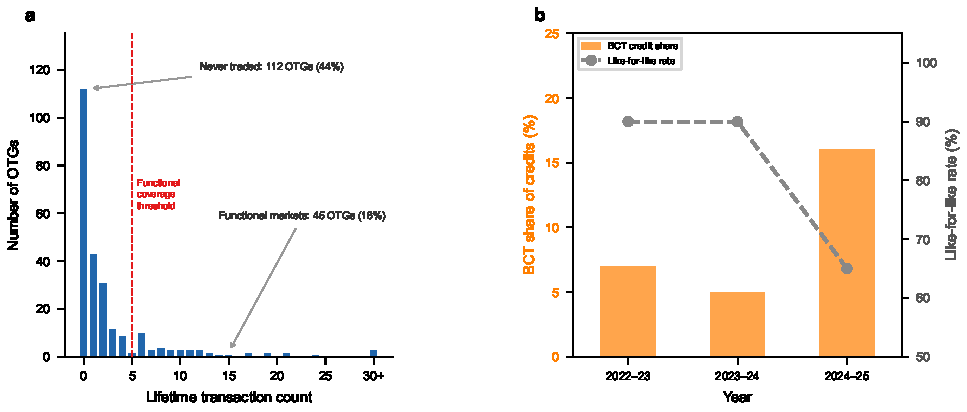
\includegraphics[width=\textwidth]{../output/figures/main/fig1_problem.pdf}
\caption{%
  \textbf{The coverage gap in the NSW biodiversity offset market.}
  \textbf{a}, Distribution of 252 ecosystem OTGs by lifetime transaction count;
  112 (44\%) have never traded; only 45 (18\%) exceed the functional
  coverage threshold of 5 transactions (red dashed line).
  \textbf{b}, BCT market share (orange bars) and like-for-like purchase rate
  (grey dashed line); share increased from 7\% to 16\% while like-for-like
  precision fell from 90\% to 65\%.
}\label{fig:problem}
\end{figure}

\begin{figure}[p]
\centering
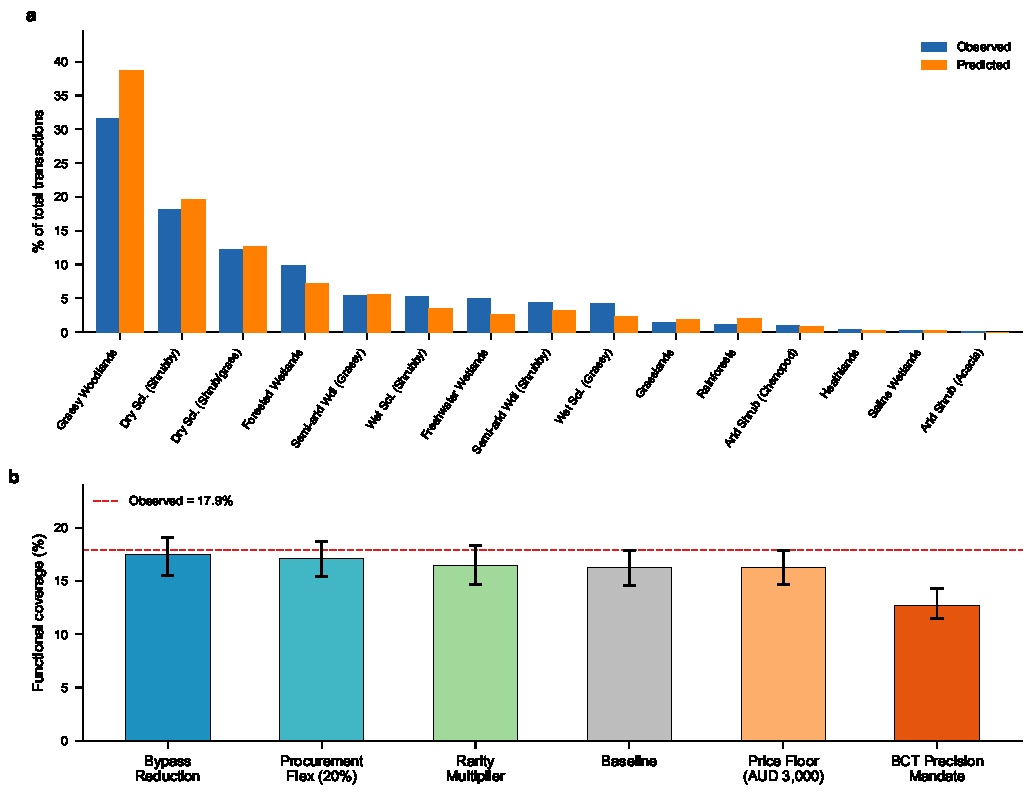
\includegraphics[width=\textwidth]{../output/figures/main/fig2_mechanism.pdf}
\caption{%
  \textbf{Formation-level model: validation and policy outcomes.}
  \textbf{a}, Observed vs predicted transaction distribution across 15
  vegetation formations (Spearman $\rho = 0.98$); the model reproduces
  the concentration of demand in Grassy Woodlands and Dry Sclerophyll
  Forests without targeting these formations during calibration.
  \textbf{b}, Functional coverage under the six policy scenarios of
  Table~1 (ABM, 50 Monte Carlo seeds; error bars: 10th--90th percentile;
  red dashed line: observed = 17.9\%). Bypass reduction and procurement
  flexibility raise coverage by keeping demand in the open market;
  price floors and the BCT precision mandate reduce it.
}\label{fig:mechanism}
\end{figure}

\begin{figure}[p]
\centering
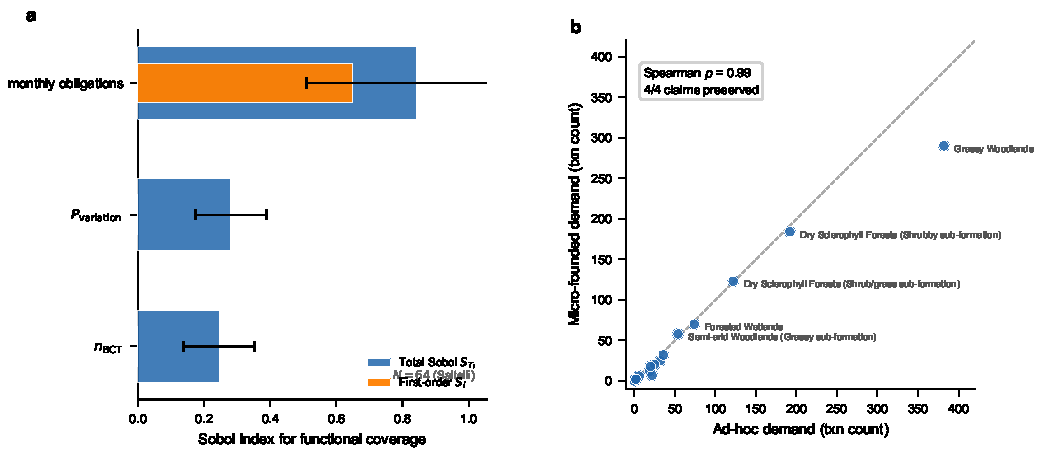
\includegraphics[width=\textwidth]{../output/figures/main/fig3_policy.pdf}
\caption{%
  \textbf{Robustness: global sensitivity analysis and demand-function
  specification.}
  \textbf{a}, Sobol indices for functional coverage as the quantity of
  interest. Total Sobol index $S_{T_i}$ (blue bars) measures the share of
  output variance attributable to parameter $i$ including all interactions;
  first-order $S_i$ (orange bars) measures the share attributable to
  parameter $i$ alone. Whiskers: bootstrap 95\% confidence intervals
  ($B = 1{,}000$). Saltelli design with $N$ base samples per parameter;
  full design and indices in Supplementary Note~2 and Supplementary
  Table~9.
  \textbf{b}, Demand-function specification test: per-formation transaction
  counts produced by the ad-hoc bid rules (horizontal axis) and the
  CARA-derived implementation (vertical axis), Spearman $\rho \geq 0.97$
  across 50 Monte Carlo seeds. The two specifications produce equivalent
  outputs at the formation level.
}\label{fig:policy}
\end{figure}


% ─────────────────────────────────────────────────────────────────────────────
% REFERENCES
% ─────────────────────────────────────────────────────────────────────────────

\bibliography{references}

\end{document}
